\newcommand{\todo}[1]{\colorbox{yellow}{\textbf{[#1]}}}
\newcommand{\wei}[1]{\textcolor{red}{{\it [Wei says: #1]}}}
\newcommand{\dan}[1]{\textcolor{blue}{{\it [Dan says: #1]}}}


\documentclass{sig-alternate}


\usepackage{cite}
%\usepackage{graphicx}
%\usepackage{hyperref}
%\usepackage{listings}
%\usepackage{times}
%\usepackage{xspace}
%\usepackage{booktabs}
%\usepackage{subfigure}
%\usepackage{fancybox}
\usepackage{color}
%\usepackage{multirow}
%\usepackage{array}
%\usepackage{subfigure}
%\usepackage{balance}
%\usepackage{tabularx}


\begin{document}

\conferenceinfo{ICSE}{'2014 Hyderabad, India}

\title{Title}



\numberofauthors{2} %  in this sample file, there are a *total*
% of EIGHT authors. SIX appear on the 'first-page' (for formatting
% reasons) and the remaining two appear in the \additionalauthors section.
%
\author{
% You can go ahead and credit any number of authors here,
% e.g. one 'row of three' or two rows (consisting of one row of three
% and a second row of one, two or three).
%
% The command \alignauthor (no curly braces needed) should
% precede each author name, affiliation/snail-mail address and
% e-mail address. Additionally, tag each line of
% affiliation/address with \affaddr, and tag the
% e-mail address with \email.
%
% 1st. author
\alignauthor
Daniel E. Krutz and Wei Le\\
       \affaddr{Rochester Institute of Technology}\\
       \affaddr{1 Lomb Memorial Drive}\\
       \affaddr{Rocheser, NY, USA}\\
       \email{\{dxkvse, weil.le\}@rit.edu}
}
% 2nd. author
%\alignauthor
%G.K.M. Tobin\titlenote{The secretary disavows
%any knowledge of this author's actions.}\\
 %      \affaddr{Institute for Clarity in Documentation}\\
  %     \affaddr{P.O. Box 1212}\\
  %     \affaddr{Dublin, Ohio 43017-6221}\\
   %    \email{webmaster@marysville-ohio.com}


\maketitle
\begin{abstract}

Developing software is hard. Developing bug free software is even more difficult. Buggy software often leads to crashes. A byproduct of these crashes are crash stacks, which is a list of all function or procedure calls which are currently in the application stack. Call stacks have become an important source for software developers to learn quality issues in released software. Since a same bug can be repeatedly triggered by different users, an overwhelming number of crash dumps are returned daily. Grouping call stacks has other advantages in the software development life cycle. Some of which include determining the cause of the issue, who should fix it, priority of a bug and even assist in intrusion detection.

In order to assist in the crash grouping process, we propose a new crash similarity measurement tool, Mozilla Call Stack Similarity (MCSS)\todo{name??} This analyzes a selected group of all stacks in a chosen application and measures the similarity of all the analyzed call stacks using several similarity measurements as defined by previous research. In the following paper, we describe this crash measurement tool along with several potential future applications of the tool. 
\todo{Really work on this abstract}

% Do any tools exist for grouping call stacks?
% What is the problem this paper is going to solve.
% How is this paper going to solve it?


\end{abstract}

% A category with the (minimum) three required fields
\category{H.4}{Information Systems Applications}{Miscellaneous}
%A category including the fourth, optional field follows...
\category{D.2.8}{Software Engineering}{Metrics}[complexity measures, performance measures]

\terms{}

\keywords{Crash Dumps, Call Stacks, Grouping, Similarity}

\section{Introduction}

Due to the complexity of software, it is unreasonable to assume that it will be created bug free in its initial release. Thus, an important and challenging task during software maintenance is to capture and diagnose failures triggered at the client side. Examples of such feedback systems include Microsoft Dr. Watson~\cite{drwatson} and Mozilla Crash Reporter~\cite{mozillacrashreporter}. In these systems, crash dumps, which typically contain call stacks recorded at the crash site, are returned for locating bugs in software. Crash or call stacks are are list of methods which have been invoked during the execution of the application which exist at the moment of the crash occurring. The most recent function call is at the top of the stack~\cite{raey}~\cite{Wang:2013:IBL:2487085.2487135}~\cite{Allwood:2009:FNS:1596638.1596654}~\cite{Seo:2012:PRC:2351676.2351702}



% Show example of a call stack in a table


Since a same bug can be repeatedly triggered by different users and under different execution environments, the number of crash dumps sent in daily can reach millions. Incorrectly grouping unrelated crash dumps or failing in identifying a new crash that actually belongs to an already fixed group can incur unacceptable manual overhead and potentially delay critical patches~\cite{6498456}~\cite{Seo:2012:PRC:2351676.2351702}. 

In order to measure the similarity of crash dumps groups from Mozilla \footnote{http://www.mozilla.org}, we developed an innovative crash measurement tool known as Mozilla Call Stack Measurment (MCSM). We decided to create a tool which analyzed Mozilla crash stacks for several reasons. First of all, there is a substantial amount of Mozilla crash data which is freely available for analysis. While there are other applications which offer significant amounts of crash information, we felt that the Mozilla suite of applications was the best to analyze because it also offered the opportunity to examine several applications, not merely a single application from a single company. Secondly, a wide range of research has been done using the Mozilla suite of applications~\cite{Dhaliwal:2011:CFC:2117694.2119726}~\cite{5298423}~\cite{6224279}~\cite{5928673}~\cite{6224281}. We wanted to develop a tool for an application suite which other researchers not only had access to a substantial amount of crash data, but also a suite which a large amount of research was also being conducted in. This would allow others to use the proposed tool for their own research.

Self managing systems that properly form crash grouping make bug fixing easier and cheaper largely due to the need for less human intervention and manual work. Determining how related two crashes are may assist with this process~\cite{raey}. Additionally, a crash similarity measurement tool may be used to place crashes into buckets, which are groups of related call stacks~\cite{Seo:2012:PRC:2351676.2351702}. These groups of related stacks are likely indicative of related crashes and related crash symptoms. Related crashes may mean that if one is fixed, all of them will be repaired as well~\cite{Dang:2012:RMC:2337223.2337364}.

% Really drive home why this tool is important
% Remember to focus on the goal for the paper.  Why is it important?

A call stack measurement tool such as the one being proposed is beneficial for several reasons. First of all, it may be used to evaluate the effectiveness of an employed call stack grouping mechanism. There are many possible ways to group call stacks. Some of which include grouping using only the signature of the stack, using heuristics for string matching such as subsequences, edit distance and prefix matching~\cite{Brodie2}~\cite{4401026} or even machine learning techniques~\cite{Bartz:2008:FSF:1855895.1855896}. Additionally, a tool such as the one being proposed could be used to augment existing techniques by providing an additional data set.


\todo{remember that we are not grouping stacks, only measuring similarity}
\todo{remember that right now, I am only measuring call stack similarity}



MCSM works with the user first selecting the target application and version. For example, the user may choose to analyze Firefox version 19.1. MCSG then scans the crash stacks for the top 300 crashes for the application. Once the call stacks are collected, they are compared against one another in a round robin fashion using call stack comparison techniques derived from the works of Modani~\emph{et al.}~\cite{4401026}, Brodie~\emph{et al.}~\cite{raey} and Bartz~\emph{et al.}~\cite{Bartz:2008:FSF:1855895.1855896}. The final results are output to a final report file. 

MCSM is the first third party tool which we are aware of which measures Mozilla crash stack similarity. Presently, Mozilla groups crashes based on the the top method signature of the crash stack. However, identical bugs may not share the same method signature, thus making such a grouping process inaccurate~\cite{Dhaliwal:2011:CFC:2117694.2119726}. The proposed tool is not only useful for measuring Mozilla crash stack similarity, but is extensible for future research. The tool is designed in such a way that new or updated call stack measurement functionality may easily be added to the system. % Remove this? What other research?

The remainder of this paper is organized as follows. Section~\ref{sec: tool} describes the created tool. Section~\ref{sec: futurework} describes future work on this project and applications of the tool. Section~\ref{sec: relatedwork} discusses related works to this paper. Section~\ref{sec: conclusion} provides a summary of this work.


% All versions of Firefox receive 600-700k crash reports a week. These are too many crash reports to be manually analyzed or grouped by developers.  ~\cite{5711013}



\section{Tool}
\label{sec: tool}

The two primary components to MCSG are the call stack data collection and call stack similarity measurement mechanisms. While the tool has been developed in Java, the described process is language agnostic and may be applied by other researchers to develop a similar tool.


\subsection{How Tool Works}

The first step of MCSG is the data collection phase. For this step, the user selects a group of crash stacks to be analyzed. This may be for a specific Mozilla application and version. For example, the user may choose to analyze all call stacks for Mozilla  22.0. MCSG will then begin to pull the emph{top crasher} call stacks for the specified application and version from the Crash Stats Mozilla website\footnote{https://crash-stats.mozilla.com/}. A top crasher is a crash type with the maximum number of crash reports~\cite{Dhaliwal:2011:CFC:2117694.2119726}.

The data collection process begins by gathering the call stacks for these top crashers. This is done using a tool known as HttpUnit\footnote{http://httpunit.sourceforge.net}. Each of the collected call stacks are stored locally in a .txt file in the folder with all the other call stacks from the same top crasher group.

% Make sure that all three of these measurement mechanisms are actually used
Once all of the folders and call stacks have been collected, the comparison process may begin. There are several existing techniques for measuring cal stack similarity~\cite{Brodie2}~\cite{Bartz:2008:FSF:1855895.1855896}~\cite{4401026}. MCSG measures call stack similarity using the call stack similarity metrics as defined in these works. If a researcher wishes to add, modify or remove a call stack similarity measurements algorithm to the tool, it is designed to make this as easy as possible.
% How is it archtectured in this manner?

% Describe how all the formulas end up getting laid out.
%Modani
% 	Describe the algorithms discussed by Modani on page 435
%	
 

% Tool and complete results are available from the tool website at: http://www.se.rit.edu/~dkrutz/MCSD/
% dhaliwal uses levensthein~\cite{citeulike:259508} distance  to evaluate distance between stacks. - Top 10 frames. - Pg 3 further describes how this evaluation takes place.


Figure~\ref{fig:toolstructure}
\begin{figure}[thb!]
\centering
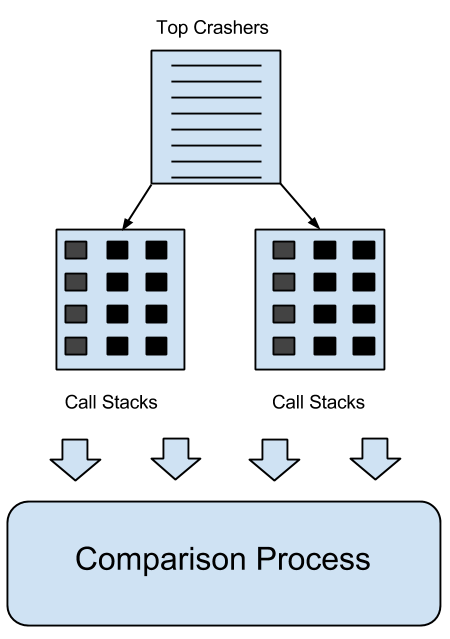
\includegraphics[width=40mm,height=70mm]{images/crashgroupingtool.png}
\caption{Overview of the tool}
\label{fig:toolstructure}
\end{figure}


\subsection{Initial Results}
Initial Results

% How does the tool work
% Where is the tool available
% Provide a diagram of the tool
% Provide some data to show that the tool actually works.
	% This will likely involve some manual verification.

% "Normal pulls" vs. random data
% Show some of these intitial results for the pulls
%  Show the comparison results for the top x "crashers"

\section{Future Work}
\label{sec: futurework}
Future Work

While MCSG works well, there is room for improvement and future work.


% Our same technique may be applied to other crash grouping tools. More analysis.
% Find a more effective grouping algorithm
% How can this relationship information be used in furture research?
% Compare manually and automatically grouped crashes 
% ? DId not do recursion removal as mentioned by Modani
% Make the comparison process go faster
% Create a better comparison algroithm
% 


\section{Related Work}
\label{sec: relatedwork}

Brodie~\emph{et al.}~\cite{Brodie2} developed the techniques of normalizing strings based on length before comparing them. They applied metrics commonly used in string matching algorithms, including edit distance, longest common subsequence and prefix match.

Brodie~et al. ~\cite{raey}, proposed that similar bugs are likely to produce stacks which resemble one another. To determine if a new failure is originated from the same cause documented in the database, they developed the metrics of Brodie weight for determining similarities between call stacks. The idea is that when measuring similarity, a higher weight is placed upon items that match between the top of two stacks. The assumption is that the closer to the top of a stack a function call is, the more relevant it is to the matching process ~\cite{Brodie2}.

Several crash grouping mechanisms have also been proposed. Bartz~\emph{et al.}~\cite{Bartz:2008:FSF:1855895.1855896} defined a similar-failure search engine to find similar failures across a large global data set. The primary use of this was to allow a developer to see if a similar failure had already been resolved. This mechanism worked from Windows failure reports in the Windows Error Reporting(WER) system.

Modani~\emph{et al.}~\cite{4401026} proposed and evaluated algorithms for using a weighted metric for efficiently and accurately matching call stacks. Recursive and uninformative function calls were removed from the stacks before comparison. Dang~\emph{et al.}~ \cite{Dang:2012:RMC:2337223.2337364} proposed a method of improving the grouping of grouping of Windows crash information received by WER called ReBucket. This used a method for clustering crash reports and was based on call stack matching. 

Wang~\emph{et al.}~\cite{Wang:2013:IBL:2487085.2487135} discussed three rules which they found could be used to automatically correlate crash types. These three criteria were a crash signature comparison, top frame comparison and a frequent closed ordered sub-set comparison. Using these criteria, the authors were able to identify crash correlation groups with a precision of between 79\% and 100\% and a recall of between 65\% and 90\%. 

Stack traces have also been examined for a variety of other uses. Feng~\emph{et al.}~\cite{1199328}  examined how call stack information could be used to assist in anomaly detection. Schroter ~emph{et al.}~\cite{5463280} concluded that stack traces in the bug reports indeed help developers fix bugs. Dhaliwal~\emph{et al.}~\cite{Dhaliwal:2011:CFC:2117694.2119726} performed an empirical analysis of crash reports for Mozilla Firefox to determine the impact of crash grouping and evaluvate the efficiency of such grouping.


\section{Conclusion}
\label{sec: conclusion}
Conclusion
%\end{document}  % This is where a 'short' article might terminate


\bibliographystyle{abbrv}

\bibliography{callstacktool} 

% That's all folks!
\end{document}


% ICSE Information
% http://2014.icse-conferences.org/demo
% Length: 4 pages
% Date: 11/22/2013


% Todo
% - Create a website for the tool (Can use the same codebase as CCCD)
% 	- Put necessary data on the website.
%	- 
% - Make sure that the tool name and acronym are updated throughout the paper.
% - 


% - Implement the various call stack comparision techniques.
% Describe how the tool may also gather and compare manually defined call stack links
%	- Clean this up in the tool.
% 

% Tool
% - Add in updated and correct distance measurements from 
% - Maybe alter tool so it can take all grouped call stacks and bucket them based on similarity
% - 
